\chapter{Background}
In this chapter, we describe about gravitational-wave and detector.

\section{Gravitational-wave}
Gravtational-wave (GW) is a ripples of the space-time, which propagates at the speed of light. GW was predicted by A. Einstein in 1918, and is a result of the general theory of relativity. However because this strain is very small, the direct discovery of GWs have not done by LIGO until 2015.

\subsection{Properties of GWs}
\subsubsection{Two polized transverse wave}
The interval between two events in space-time is
described with the metric tensor $g_{\mu\nu}$ as, 
\begin{eqnarray}
  d s^{2}=g_{\mu \nu} d x^{\mu} d x^{\nu} (\mu,\nu = 0,1,2,3),
\end{eqnarray}
where $dx^{\mu}$ represents the coordinate distance of the events, and $x^{\mu}$ has 4 components; $(ct,x,y,z)$.

In the general relativity theory\cite{einstein1916vd}, the metric tensor $g_{\mu\nu}$ is described by the Einstein's equation;
\begin{eqnarray}
  R_{\mu \nu}\left(g_{\mu \nu}\right)-\frac{1}{2} g_{\mu \nu} R\left(g_{\mu \nu}\right)=\frac{8 \pi G}{c^{4}} T_{\mu \nu},
\end{eqnarray}
where $R_{\mu\nu}$ is the Ricci tensor, $R=g^{\mu \nu} R_{\mu \nu}$ is the Ricci scalar curvature, $T_{\mu\nu}$ is the energy-momentum tensor, $G$ is the Newton's gravitational constan, and $c$ is the speed of light.

GW is derived from this Einstein's equation when the metric can be described as the perturbation $h_{\mu\nu}$ to the Minkowsky space-time $\eta_{\mu\nu}$, thus
\begin{eqnarray}
  g_{\mu \nu}=\eta_{\mu \nu}+h_{\mu \nu}.
\end{eqnarray}
In this weak-field regime, the Einsteins's equation is reduced to a linearized wave-equation whose solution is represented as
\begin{eqnarray}
  h_{\mu \nu}(z, t)=\left(\begin{array}{cccc}{0} & {0} & {0} & {0} \\ {0} & {-h_{+}} & {h_{\times}} & {0} \\ {0} & {h_{\times}} & {h_{+}} & {0} \\ {0} & {0} & {0} & {0}\end{array}\right) \cos \left[\omega\left(\mathrm{t}-\frac{\mathrm{Z}}{\mathrm{c}}\right)\right],
\end{eqnarray}
where $\omega$ is the angluar frequency of GW, $z$ is the propagation direction of the wave, $h_{+} \text {and } h_{\times}$ are the independent polization of that. Therefore, GW is the transverse wave propagating with speed of light.

The two polization of GW are known as plus and cross polization, and these polization change the distance between two points as shown in Fig.\ref{img:img131}. 

\begin{figure}[h]
  \begin{center}   
    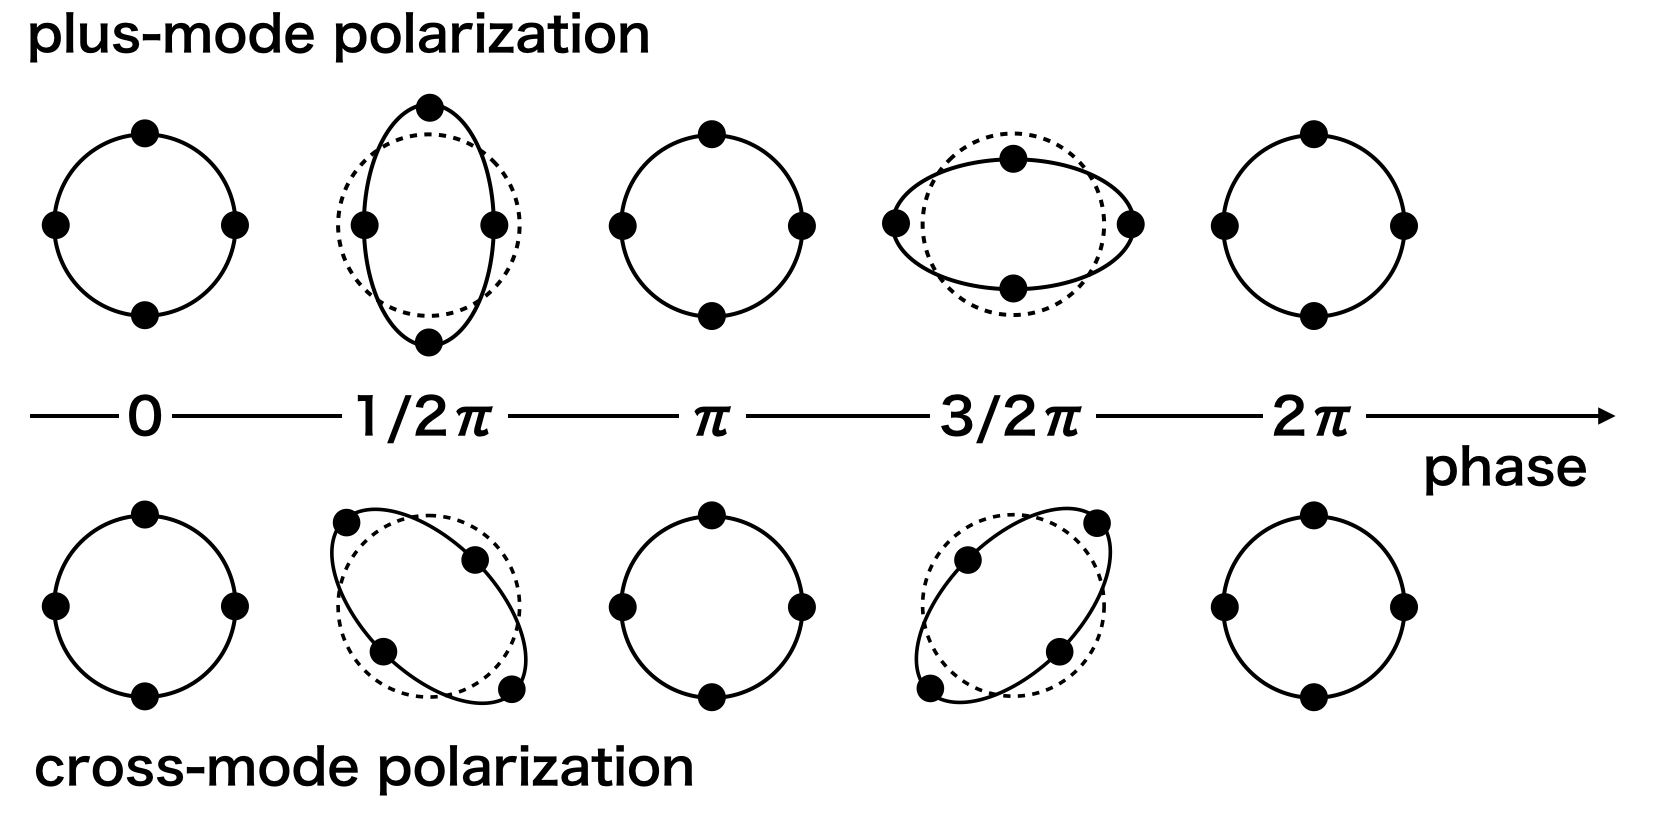
\includegraphics[width=11.0cm]{./img_chap1/img131.png}
    \caption[Polization of the GW]{Polization of the GW propagating in the direction of the paper. These polization change the distance as the tidal motion.
}\label{img:img131}
  \end{center}
\end{figure}

%% \subsubsection{Radiation}
%% The wave amplitude $h_{\mu\nu}$ is proportional to the second time derivative of the quadrupole moment of the source \cite{einstein1918gravitationswellen};
%% \begin{eqnarray}
%%   h_{i j}=\frac{2}{r} \frac{G}{c^{4}} \ddot{Q}_{i j}^{T T}\left(t-\frac{r}{c}\right),
%% \end{eqnarray}
%% where 
%% \begin{eqnarray}
%%   Q_{i j}^{T T}(x)=\int \rho\left(x^{i} x^{j}-\frac{1}{3} \delta^{i j} r^{2}\right) d^{3} x
%% \end{eqnarray}
%% is the quadrupole.

%% \textcolor{red}{もうすこし具体的なQuadrupoleをしめして、現実的に検出できそうな重力波の大きさを述べる。}

\subsection{Sources of Gravitational-wave}
\subsubsection{Compact Binary Coalescence}
Compact binary coalescence (CBCs), such as black holes and neutron stars, emit a characteristic chirp GW signal. The frequency of a hirp GW signal $f_{g}$ increase as a function of time. This growing up is caused by loosing the angluar momentum of the system due to the emittion of GW. 

Advanced LIGO have detected the first GWs from stellar-mass binary black holes (BBHs) in the first observation run (O1), which took place from September 12, 2015 until January 19, 2016. After this observation, Virgo detector joined the Advanced LIGO detectors and this network have detected the first detection of GWs from a binary neutron star inspiral in the second observation run (O2), which ran from November 30, 2016 to August 25, 2017. Moreover, observation of GWs from a total of seven BBHs \cite{abbott2019gwtc}.


\subsubsection{Continuous GWs}
Without rotating two objects, asymmetric spinning stars, such as neutron stars and pulsars, could produce detectable GWs which signal is also well defined \cite{leaci2012searching,hereld1984search}.

\subsubsection{Burst GWs}
In addition to continuous gravity waves, there are short suration GWs like a burst event. Supernovae are good candidates to emit te burst GWs \cite{ott2004gravitational}

\subsubsection{Stochastic GWs}
The stochastic background GWs are predicted\cite{starobinskii1979spectrum,Christensen_2018}. This background signal is originated from quantum fluctuations during inflation \cite{PhysRevD.23.347}. Basically, stochastic bacground will appear like a random noise in an individual detector. However, it will be found like a coherent signal in two detector.

%\cite{damour2005gravitationa}




\section{Interferometric Gravitational-wave detection} \label{sec:12}
Basic design of a terrestrial GW detectors are Michelson interferometer \cite{weiss1972electronically}. This interferometer sensitives to the differential length change of its arms. This change is a strain caused by GWs. We assume that puls mode of GW is passing thorugh the interferometer perpendicularly.

\subsection{Michelson Interferometer} \label{sec:121}
\begin{figure}[h]
  \begin{center}   
    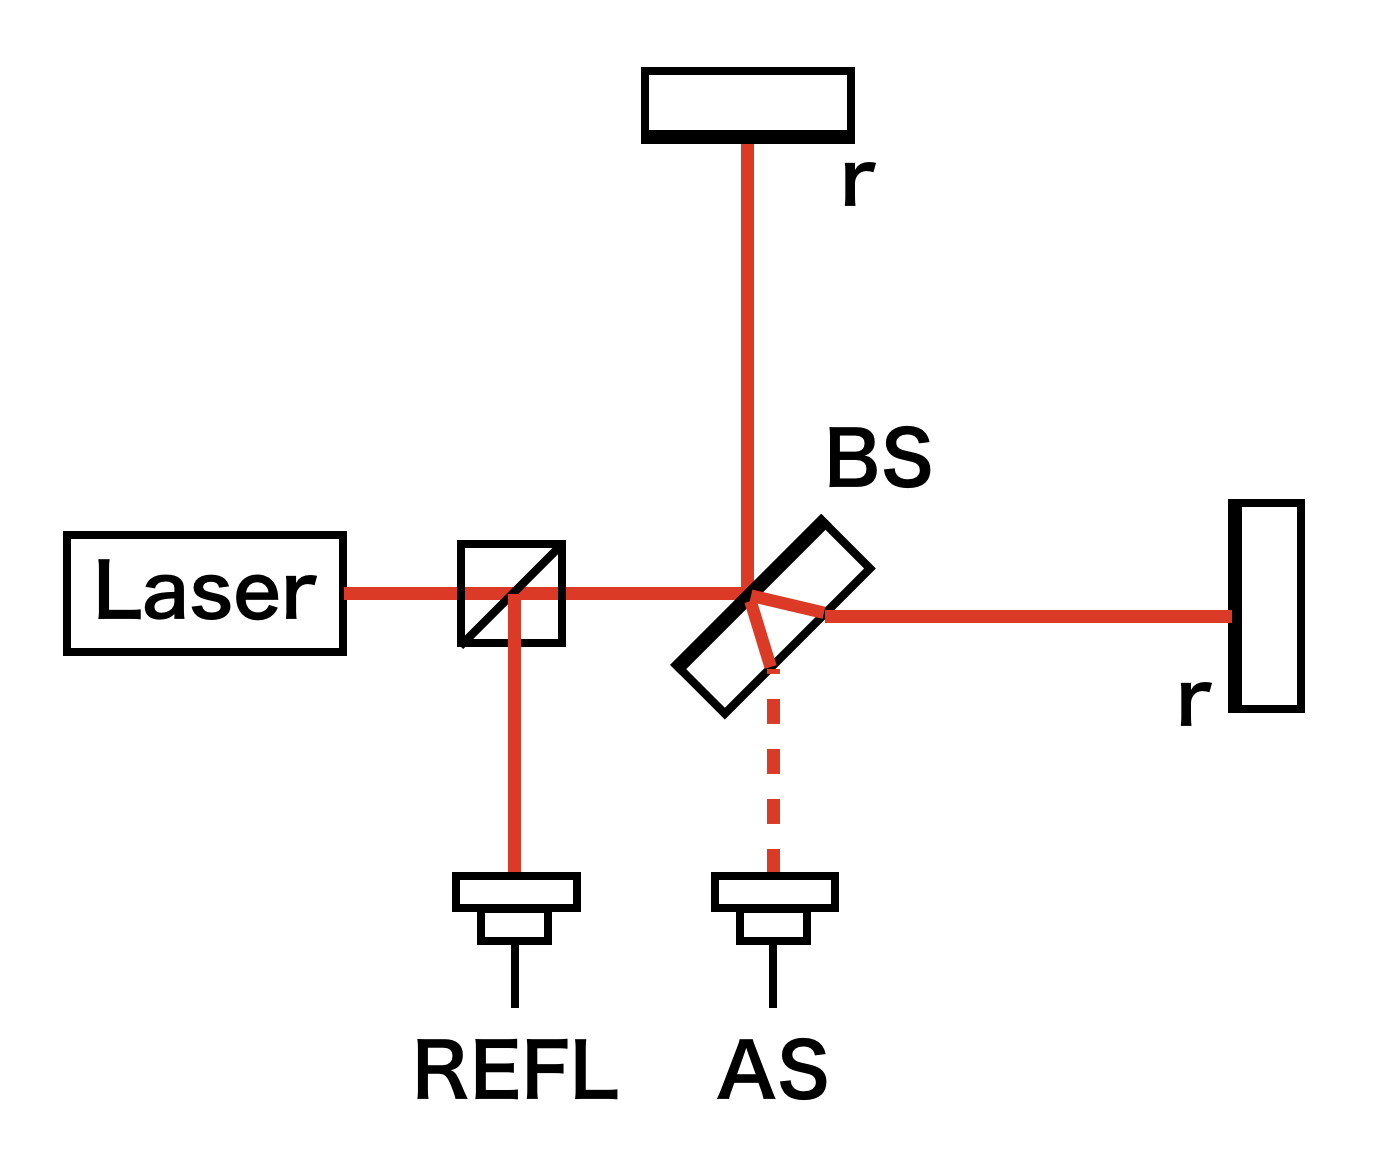
\includegraphics[width=8.0cm]{./img_chap1/img132.png}
    \caption{Michelson Interferometer. }\label{img:img132}
  \end{center}
\end{figure}

Michelson interferometer is a converter from the optical phase difference of two lights to the amplitude modulation of a single light. Consider about the interferometer shown in Fig. \ref{img:img132}. Incident light can be wrtten as,
\begin{eqnarray}
  E_{\mathrm{in}} = E_{0} e^{i\omega{t}},
\end{eqnarray}
where $E_0$ is the amplitude and $\omega_0$ is the angular frequency of the laser field
. Two lights splited by the Beam Spliter (BS) interferer at the Anti-symetric (AS) port and Refrection (REFL) port. The output fieled at the AS port is represented as,
\begin{eqnarray}
  E_{\mathrm{AS}} = -\frac{1}{2}rE_{0} e^{i\left(\omega_{0} t-\phi_{x}\right)}+\frac{1}{2}r E_{0} e^{i\left(\omega_{0} t-\phi_{y}\right)},
\end{eqnarray}
where $r$ denote the amplitude reflectivity of the end mirrors, and $\phi_{x}$ and $\phi_{x}$ are the phase delay due to the light traveling in the $x$ and $y$ arms. This output signal can be represented as a single fieled as,
\begin{eqnarray}
E_{\mathrm{AS}} = i r E_{0} e^{i\left(\omega_{0} t-\left(\phi_{x}+\phi_{y}\right) / 2\right)} \sin \left(\frac{\phi_{x}-\phi_{y}}{2}\right). \label{eq:eq132}
\end{eqnarray} 
Wwe find that the amplitude of the output light is a function of the difference between two phases; $\phi_{x}-\phi_{y}$. Furthermore, the power of output light at the AS port is obtained by squaring the Eq.\ref{eq:eq132}, 
\begin{eqnarray}
  P_{\mathrm{AS}} &=\left[r\sin({\phi_{-}})\right]^2P_0  \label{eq:eq133}
\end{eqnarray}
Similarly, power of the output light as REFL port is written as,
\begin{eqnarray}
  P_{\mathrm{REFL}} &=\left[(r\cos({\phi_{-}}))\right]^2P_0. \label{eq:eq134}
\end{eqnarray}
Therefore, we can measure the optical phase difference as the amplitude changes using a Photo Detector (PD) and detect GWs.

\subsection{Static Response}
Consider the error of the interferometric strain measurement. Bacause the optical phase $\phi_{-}$ is given by
\begin{eqnarray}
  \phi_{-}=\frac{4\pi{L_{-}}}{\lambda},
\end{eqnarray}
where $L_{-}$ is the differential length changes of its arms and $\lambda$ is the wavelength of the input laser, the strain $h$ is represented as 
\begin{eqnarray}
  h = \frac{\Delta{L_{-}}}{L} = \frac{\lambda}{4\pi{L}}\Delta{\phi_{-}} + \frac{L_{-}}{L}\left(\frac{\Delta{f}}{f}\right). \label{eq:eq133_a}
\end{eqnarray}
Moreover, according to Eq.(\ref{eq:eq133}), because infinitesimal change of the optical phase $\Delta{\phi_{-}}$ is given by 
\begin{eqnarray}
  \Delta{\phi_{-}} = \frac{\tan{(\phi_{-})}}{2} \left[\left(\frac{\Delta P_{\mathrm{AS}}}{P_{\mathrm{AS}}}\right) + \left(\frac{\Delta{P_0}}{P_0}\right) \right],
\end{eqnarray}
where $\Delta{P_0}$ is the fluctuation of the input laser and $\Delta{P_{\mathrm{AS}}}$ is a power fluctuation at AS port, finaly, we get a strain as a function of several fluctuation of parameters below;
\begin{eqnarray}
  h = \frac{\lambda}{8\pi{L}}\tan{(\phi_{-})} \left[\left(\frac{\Delta P_{\mathrm{AS}}}{P_{\mathrm{AS}}}\right) + \left(\frac{\Delta{P_0}}{P_0}\right) \right] + \frac{L_{-}}{L}\left(\frac{\Delta{f}}{f}\right). \label{eq:eq137b}
\end{eqnarray}

According to Eq.(\ref{eq:eq137b}), in order to increase the interferometric strain measurement, we should do below;
\begin{itemize}
  \setlength{\itemsep}{1pt}      %2. ブロック間の余白
  \setlength{\parskip}{-1pt}     %4. 段落間余白.
  \setlength{\itemindent}{0pt}   %5. 最初のインデント
  \setlength{\labelsep}{5pt}     %6. item と文字の間
\item we should expand the baseline length $L$.
\item we should operate the Michelson intereferometer at dark fringe, which means $\phi_{-}\to0$, in order to decrease the noise contribution from $(\Delta P_{\mathrm{AS}}/P_{\mathrm{AS}})$ and $\Delta{P_0}/P_0$ to the strain $h$.
\item we should use asymmetric arm so that $L_{0}\to0$, in order to decrease the noise contribution from the laser frequency fluctuation $\Delta{f}{f}$
\end{itemize}

\newpage
\section{Enhancement of the sensitivity}
\begin{figure}[h]
  \begin{center}   
    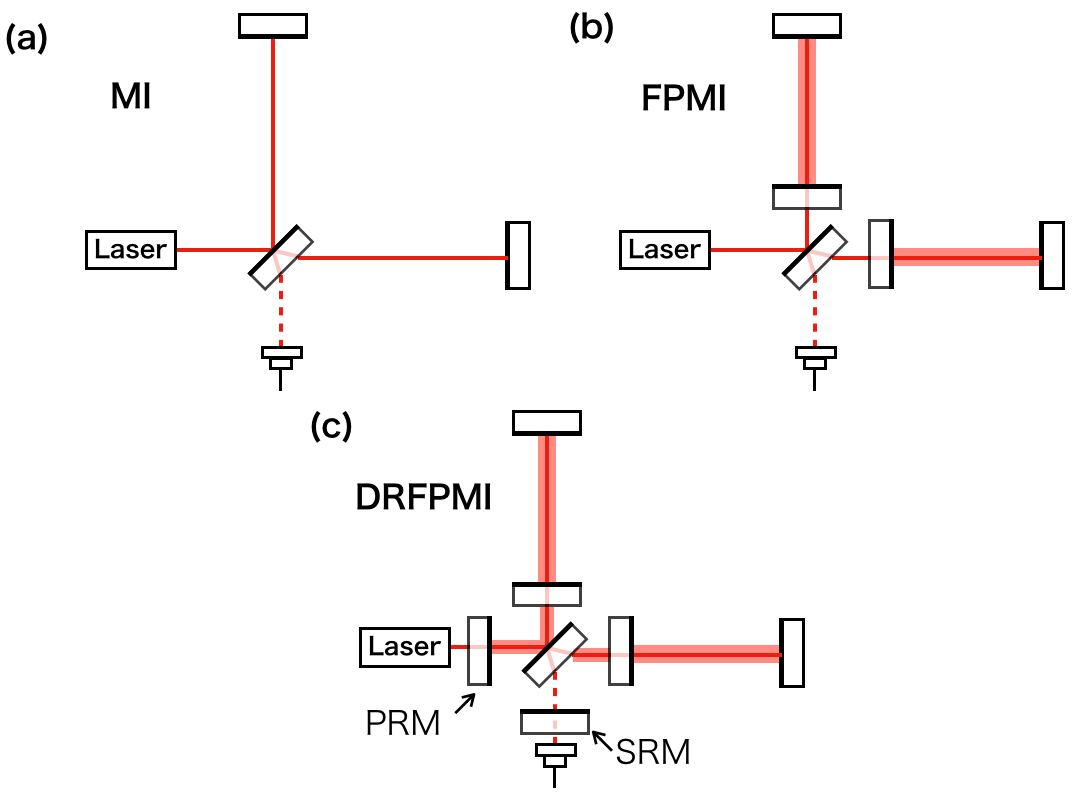
\includegraphics[width=14cm]{./img_chap1/img133.png}
    \caption{Configuration of interferometric GW detector. (a) Michelson interferometer (MI) (b) Michelson interferometer with two Fabry-Perot optical cavities (FPMI). (c) Dual-Recycled FPMI (DRFPMI)} \label{img:img133}
  \end{center}
\end{figure}
In order increase the sensitivity, current interferometric GW detector use the Dual-Recycled Fabry-Perot Michelson Interferometer (DRFPMI). 


\subsection{Fabry-Perot Michelson Interferometer (FPMI)}

\subsubsection{Fabry-Perot Optical Cavity}
Fabry-Perot optical cavity increase the effective baseline linegth. Consider the Fabry-Perot optical cavity composed of two mirrors separated by L as shown in Fig.\ref{img:img133a}. In this figure, $E_{\mathrm{in}},\,E_{\mathrm{r}},\,E_{\mathrm{t}},\,E$ are the incident, reflected, and transmitted fields respectively, $r_{j}$ and $t_{j}$ are the amplitude reflectivity and transsivity of $j$-th mirrors ($j=1,2$). The averaged bounce number in a Fabry-Perot cavity $\mathcal{N}_{\mathrm{FP}}$ is written as \cite{ando1999power}
\begin{eqnarray}
  \mathcal{N}_{\mathrm{FP}} = \frac{2\mathcal{F}}{\pi},
\end{eqnarray}
where $\mathcal{F}$ is a finesse given as
\begin{eqnarray}
  \mathcal{F}=\frac{\pi \sqrt{r_{1} r_{2}}}{1-r_{1} r_{2}}.
\end{eqnarray}
However, in order to resonate the optical cavity, the displacement of the cavity length within linewidth calculated as the width at half maximum (FWHM) 
\begin{eqnarray}
  L_{\mathrm{FWHM}} = \frac{\lambda}{2\mathcal{F}}\label{eq:eq131}.
\end{eqnarray}


\begin{figure}[h]
  \begin{minipage}[b]{0.5\hsize}
    \begin{center}   
      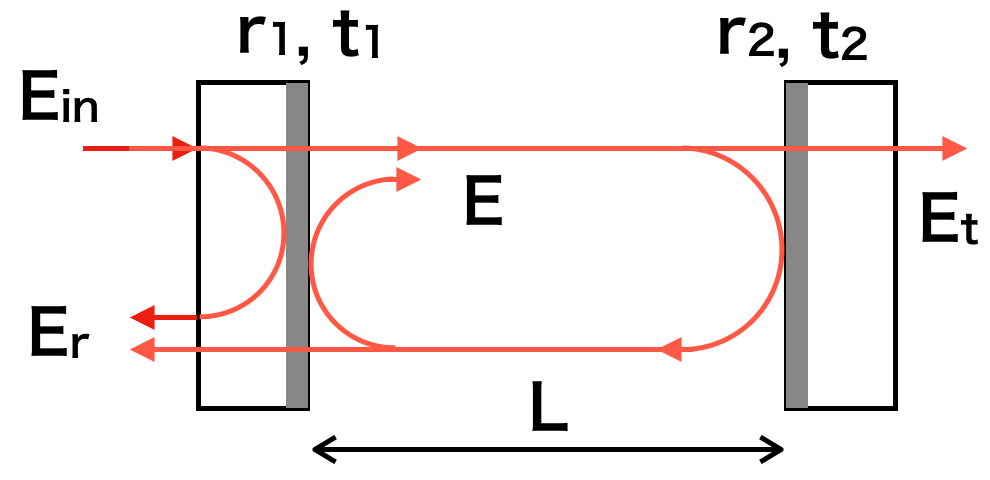
\includegraphics[width=7cm]{./img_chap1/img133a.png}
      \subcaption{Fabry-Perot optical cavity composed of two mirrors separated by L. } \label{img:img133a}
    \end{center}
  \end{minipage}\hspace{3pt}
  \begin{minipage}[b]{0.5\hsize}
    \begin{center}   
      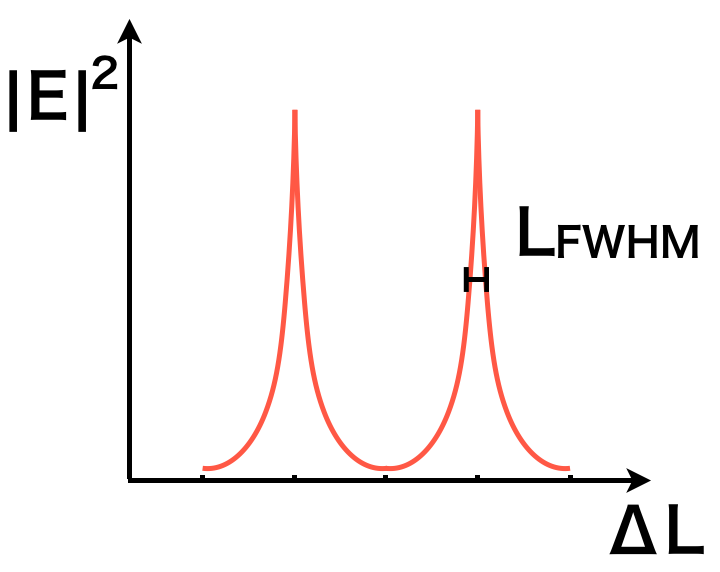
\includegraphics[width=5cm]{./img_chap1/img133b.png}
      \subcaption{Intra-cavity power as a function of displacement of cavity length.} \label{img:img133b}
    \end{center}    
  \end{minipage}
  \caption{Fabry-Perot optical cavity.}
\end{figure}


\subsection{Dual-Recycled FPMI (DRFPMI)}
As shown in Fig.\ref{img:img133}(c), final configuration of the current GW is DRFPMI which has two recycling optical cavity \cite{meers1988recycling}.

\subsubsection{Power Recycle}
In order to decrease shot noise, power recycling technique is used. In this technique, additional mirror is installed between laser and interferometer to increase the effective laser power by recycling the reflected light from the interferometer. Increaseing the laser power, the noise to signal ratio of shot noise is decrease as mentioned later.

\subsubsection{Signal Recycle}
Signal recycling mirror, which is installed on the AS port, is for tunning the frequency band. This mirror enhance the GW signal by recycling the output signal from the interferometer.

\subsection{Noise}
In terms of the interferometric GW detector, noise can be classified into two noises; detection noise and displacement noise of the testmass.

\subsubsection{Shot Noise}
In an ideal case that the test mass is not disturbed and as the free mass, the noise of the interferometer is limited by the shot noise.

Shot noise is a noise associated with the fluctuation of the number of photons at the photo detector. In case that the number of photons $N$ are large enough ($N\gg1$), the number of photon obey the Gaussian distribution with standard deviation of $\sqrt{N}$. Therefore, if laser power $P$ incidents in the detector, shot noise has a relation with the power;
\begin{eqnarray}
  P_{\mathrm{shot}} \propto \sqrt{P}\ \ [W/\sqrt{\mathrm{Hz}}].  \label{eq:eq136}
\end{eqnarray}
One can find that shot noise is a white noise, which propotional to the square-root of the incident power.

Here, according to Eq.(\ref{eq:eq133}), relative error of power at the detector is given by 
\begin{eqnarray}
  \frac{\Delta P_{\mathrm{AS}}}{P_{\mathrm{AS}}}  \propto \frac{1}{\sqrt{P_{\mathrm{0}}}}\ \ [1/\sqrt{\mathrm{Hz}}],  \label{eq:eq136}
\end{eqnarray}
where $P_{\mathrm{AS}},\,\Delta P_{\mathrm{AS}}$ are the power at the photo detector, $P_0$ is the power of the incident beam. This shows that we increasing the input power can decrease the shot noise.

\subsubsection{Seismic Noise}
Seismic noise is the largest displacement noise for interferometric GW detector. Seismic waves from various excitation sources disturbe the test mass through the mechanical structures. Therefore, in order to reduce the seismic noise, it is necessary to suspend the test masses far from the excitation sources. More details are described in the next chapter.

\subsubsection{Newtonian Noise}
Unlike the seismic noise mentioned above, the Newtonian noise is a noise that the density fluctuation of surrounding objects disturbes the test mass by gravitational interaction. Because this noise propagate through space, it can not isolate by using the vibration isolation scheme. Although the noise does not affects on the current 2nd generation GW detectors, it will contamintate on the next 3rd generation detectors.

In order to reduce the Newtonian noise, the feedforward control using the seismometer array is proposed.

\subsubsection{Thermal Noise}
In addition to external disturbances such as the seismic origin noise, the mirror substrate and surface particles cause random thermal motion generate displacement noise. This thermal noise can be classified into two; 1) mirror thermal noise 2) mirror coating thermal noise \cite{dan2016study}.

The displacement noise of the mirror thermal noise of the mirror with temperature $T$ is given by \cite{levin1998internal,numata2003wide}
\begin{eqnarray}
  G_{\mathrm{SB}}(f)=\frac{4 k_{B} T}{\omega} \frac{1-\sigma^{2}}{\sqrt{\pi} E w_{0}} \phi_{\mathrm{sub}}(f),
  \label{eq:eq140}
\end{eqnarray}
where $k_{B}$ is a Boltzmann constant, $\omega$ is angular frequency, $\sigma,\,E,\, \phi_{\mathrm{sub}}$ are a Poisson's ratio, Young's modulus, and mechanical loss angle of the bulk of the mirror respectively, and $\omega_0$ is a beam radius. One can find that the mirror thermal noise is decreased by lower temperature or increase the beam radius.

The displacement noise of coating thermal noise is given by \cite{numata2003wide,harry2002thermal}
\begin{eqnarray}
  G_{\mathrm{CB}}(f)=G_{\mathrm{SB}}(f)\left(1+\frac{2}{\sqrt{\pi}} \frac{1-2 \sigma}{1-\sigma} \frac{\phi_{\mathrm{coat}}}{\phi_{\mathrm{sub}}} \frac{d}{w_{0}}\right), 
\end{eqnarray}
were $d$,$\phi_{\mathrm{coat}}$ are depth and loss angle of the coating.


\newpage
\section{Large-scale Terrestrial Laser Interferometers}
Large-scale baseline is a essential feature of interferometric GW detectors for improving the sensitivity. 

\subsection{Terrestrial Laser Interferometers}
So far, various interferometric GW detectors are developed in many places. These detectors are listed table \ref{tb:tb101}.

\begin{table}[h] 
  \begin{center}
    \caption{Terrestrial laser interferometers \cite{chen2017brief,beker2013low}}\label{tb:tb101}
    \begin{tabular}{llll} 
      \hline
      Generation &Project & Baseline [m] & Bedrock \\ \hline \hline
      1st &LISM  & 10    & Granite/gneiss \\ 
      &CLIO  & 100   & Granite/gneiss \\
      &TAMA  & 300   & Sedimentary soil \cite{1970449}\\ 
      &GEO   & 600   & Sedimentary rock \\ \hline
      2nd &aLIGO L1 & 4000  & Sedimentary soil \\
      &aLIGO H1 & 4000  & Sedimentary rock \\
      &aVirgo   & 3000  & Sedimentary rock \\
      &KAGRA   & 3000  & Granite/gneiss \\ \hline
      3rd &ET      & 10000 & Granite/gneiss (Planning) \\
      \hline
    \end{tabular}
  \end{center}
\end{table}


\subsubsection{1st Generation}
The first generation GW detectors (LISM \cite{sato2004ultrastable}, CLIO \cite{ohashi2003design}, TAMA \cite{ando2001stable}, GEO \cite{grote2010geo}) are small-scale detectors and for test-bench of next generation detectors.
% LIGO\cite{abbott2009ligo}, Virgo\cite{accadia2012virgo}

\subsubsection{2nd Generation}
The second generation GW detectors (KAGRA\cite{akutsu2018kagra}, Advanced Virgo\cite{acernese2014advanced}, Advanced LIGO\cite{aasi2015advanced}) are first large-scale detectors for the enough sensitivity to detect GW signal.

\subsubsection{3rd Generation}
The third generation GW detector (now ET is proposed) has a few km-scale detectors.

%% \subsubsection{LISM}
%% LISMは世界で初めて地下に建設された20mのレーザー干渉計型の重力波検出器をつかって、干渉計の安定した運転を地下環境で実証するプロジェクトである。LISMの干渉計は20mのFabry-Perot光共振器を腕にもつマイケルソン型レーザー干渉計である。この腕共振器のフィネスは25000と非常に大きくCavity Pole は150Hzに相当する。このようにフィネスの大きい共振器にもかかわらず、DutyCycleは$99.8\,\%$であった。

%% 安定稼働の大きな要因としては地面振動の同相雑音除去効果が考えられる。Fig.\ref{img:img122}にLISMの感度曲線を示す。懸架システムの伝達関数をもちいて計算された干渉計への地面振動の寄与と比較すると、地面振動の垂直方向成分が100Hz以下の感度を制限していることがわかるが、特筆すべきは6Hz以下の干渉計の感度が地面振動の寄与よりも小さいことである。これは、神岡の地下岩盤が十分に固く、低周波では20mの基線を一枚岩のようにうごかし基線長が低減される。このおかげで腕共振器が安定してロックでき、安定した干渉計の稼働が実現できた。
%% \begin{figure}[h]
%%   \begin{center}   
%%     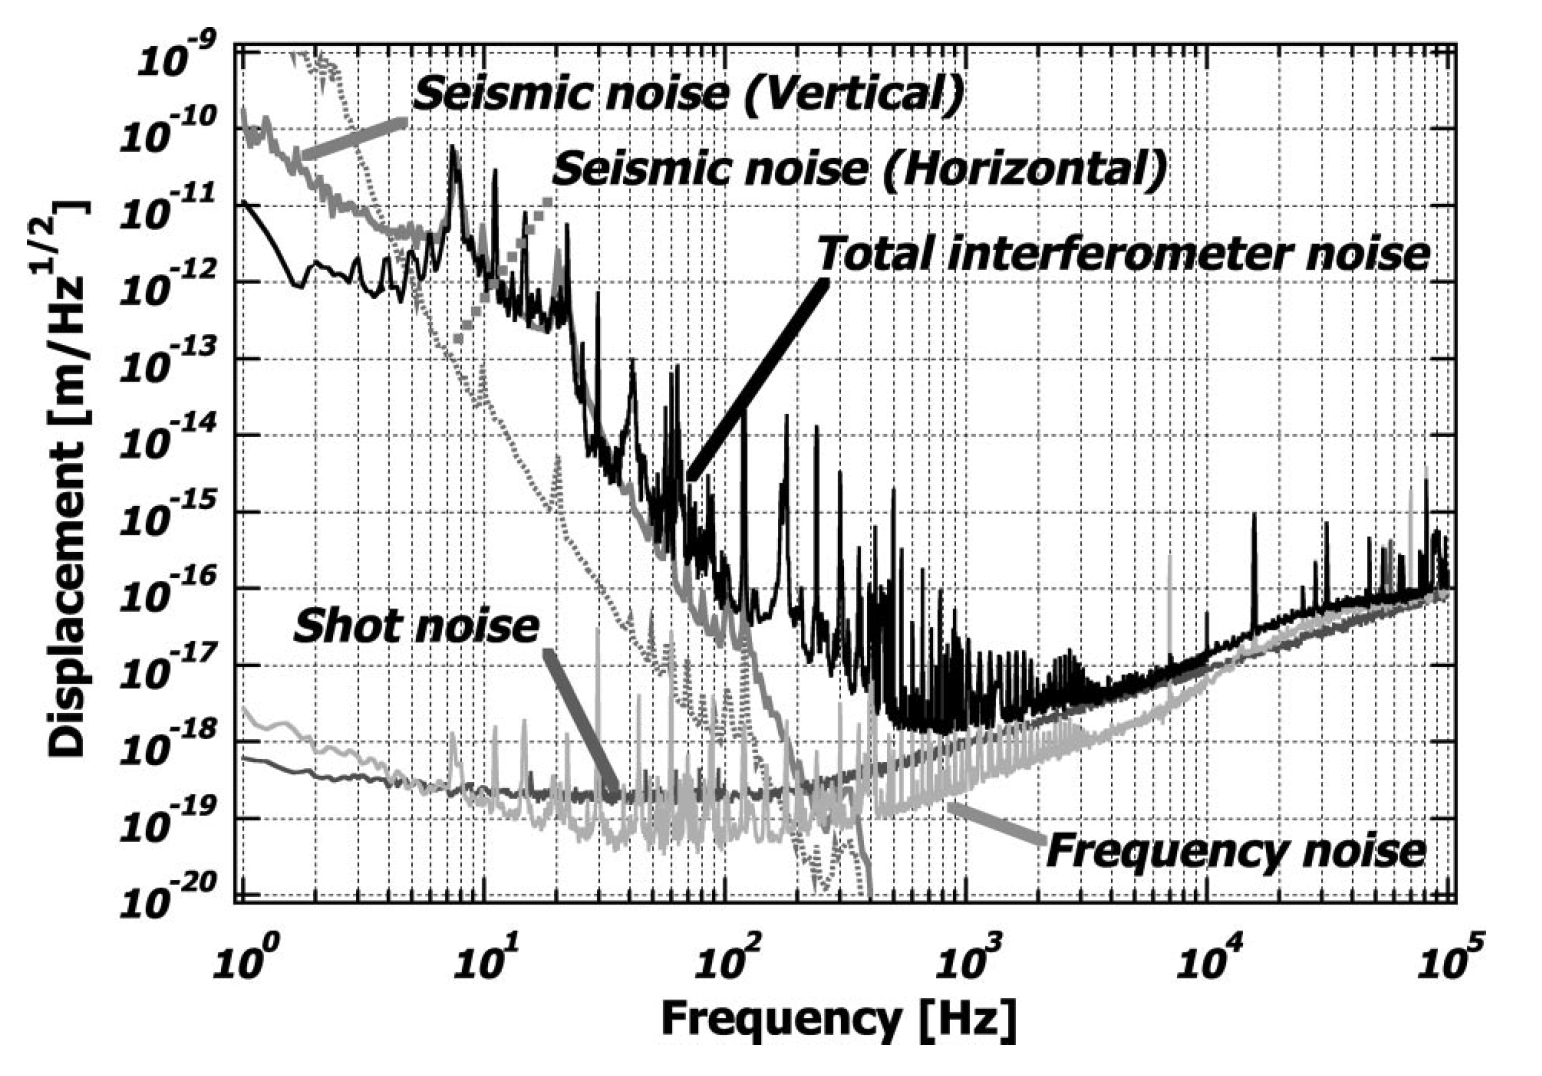
\includegraphics[width=12cm,height=7cm]{./img_chap1/img122.png}
%%     \caption{The noise equivalent detector sensitivity of LISM. This figure is cited from figure 5 in \cite{sato2004ultrastable}. } \label{img:img122}
%%   \end{center}
%% \end{figure}

%% \subsubsection{CLIO}
%% CLIOは、LISMに引き続いて地下に建設された100mのレーザー干渉計型重力波検出器であり、この検出器の目的は極低温に冷やした鏡を用いて熱雑音の低減を実証することである\cite{ohashi2003design}。そのために、地面振動が静かな地下環境で、熱伝導特性の良いサファイアでFabry−Pert光共振器を構築し、低振動なパルス管冷凍機\cite{tomaru2004development}を使用して20Kまで冷却をしている。このおかげで、室温での熱雑音で制限されていた干渉計の感度を低音鏡にして低減することができた\cite{uchiyama2012reduction}。

%% \begin{figure}[h]
%%   \begin{center}   
%%     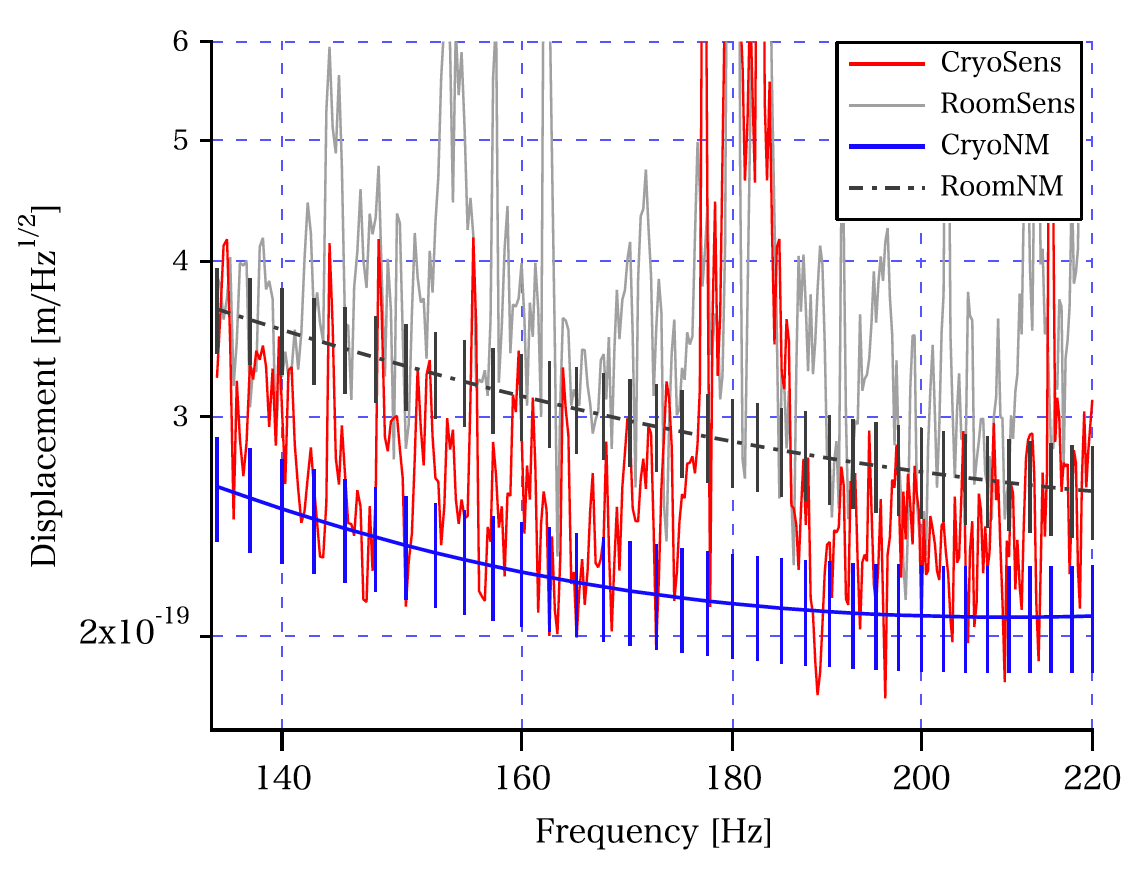
\includegraphics[width=12cm,height=7cm]{./img_chap1/img123.png}
%%     \caption{This figure is cited from figure 2 in \cite{uchiyama2012reduction}. } \label{img:img123}
%%   \end{center}
%% \end{figure}

\subsection{Degradation of duty cycle }
Large-scale baseline makes it difficult to keep the long arm cavity at the resonant state because low-frequency seismic noise disturbs the baseline length.

In case the short-scale baseline, the low-frequency seismic noise did not disturb the baseline length because the motion move the arm cavity as a singl object. However, in case the long-scale baseline, the seismic motion below $1\,\mathrm{Hz}$ move the two mirrors of the arm cavity with no correlation. Especially around $0.2\,\mathrm{Hz}$, amplitude of microseisms caused by ocean activities are larger than the linewidth of arm cavity. This means that the duty cycle of interferometric GW detectors are limited by these low-frequencies.

\subsection{Improvement of duty cycle}
Low-frequency seismic noise potentilally cause the lock acquisition failure or lock loss. 

\subsubsection{Arm length stabilization (ALS)}
ALS is a technique to reduce the RMS of arm cavity length using frequency-doubled auxiliary lasers before locking the cavity using main laser \cite{mullavey2012arm,izumi2012multi}. The wavelength of this auxliliary laser is half of the main infrared laser ($1064\,\mathrm{nm}$), thus linewidth is also half according to Eq.(\ref{eq:eq131}). This means that the auxiliary laser is more easy to lock the arm cavity than the main laser. Therefore, onece locking the arm cavity using auxiliary laser, ALS system can reduce the RMS of arm cavity length fluctuation using the feedback signal of the auxiliary system so that the main laser can lock the arm caivty. Owing to this system, lock aquisition takes less than 10 minutes.

\subsubsection{Early earthquake alert}
Although ALS system can bring the interferometer to the observation state in a sufficiently short time, this is used in only the lock aquisition phase not observation phase due to the control noise. In the obseravtion phase, we can only use the main laser with narrow linewidth as a sensor for measurering the baseline length. Moreover, we have to use a narrow dynamic range and weak actuator not to contaminate the GW sensitivity with the actuator noise. In this situation, if disturbance will excess the range of sensors and actuators, the cavity can not keep the locking state. 

Actually, duty cycle of GW detectors are limited by the low-frequency seismic noise in which the vibration isolation system could not attenuate the motion. Especially long period earthquake limites the duty cycle \cite{Biscans2018control}. 


\section{Outline of thesis}
本論文では、長期線化によって引き起こされるDutyCycleの低下についての考察と、それを解決する防振システムの開発が述べられている。


\section{Summary of the Chapter}
